\documentclass{article}
\usepackage{tikz,times}
\usepackage[paperwidth=25cm,paperheight=22cm,left=1cm,top=1cm]{geometry}

\usetikzlibrary{mindmap,backgrounds}

\pagestyle{empty}

\begin{document}
\centering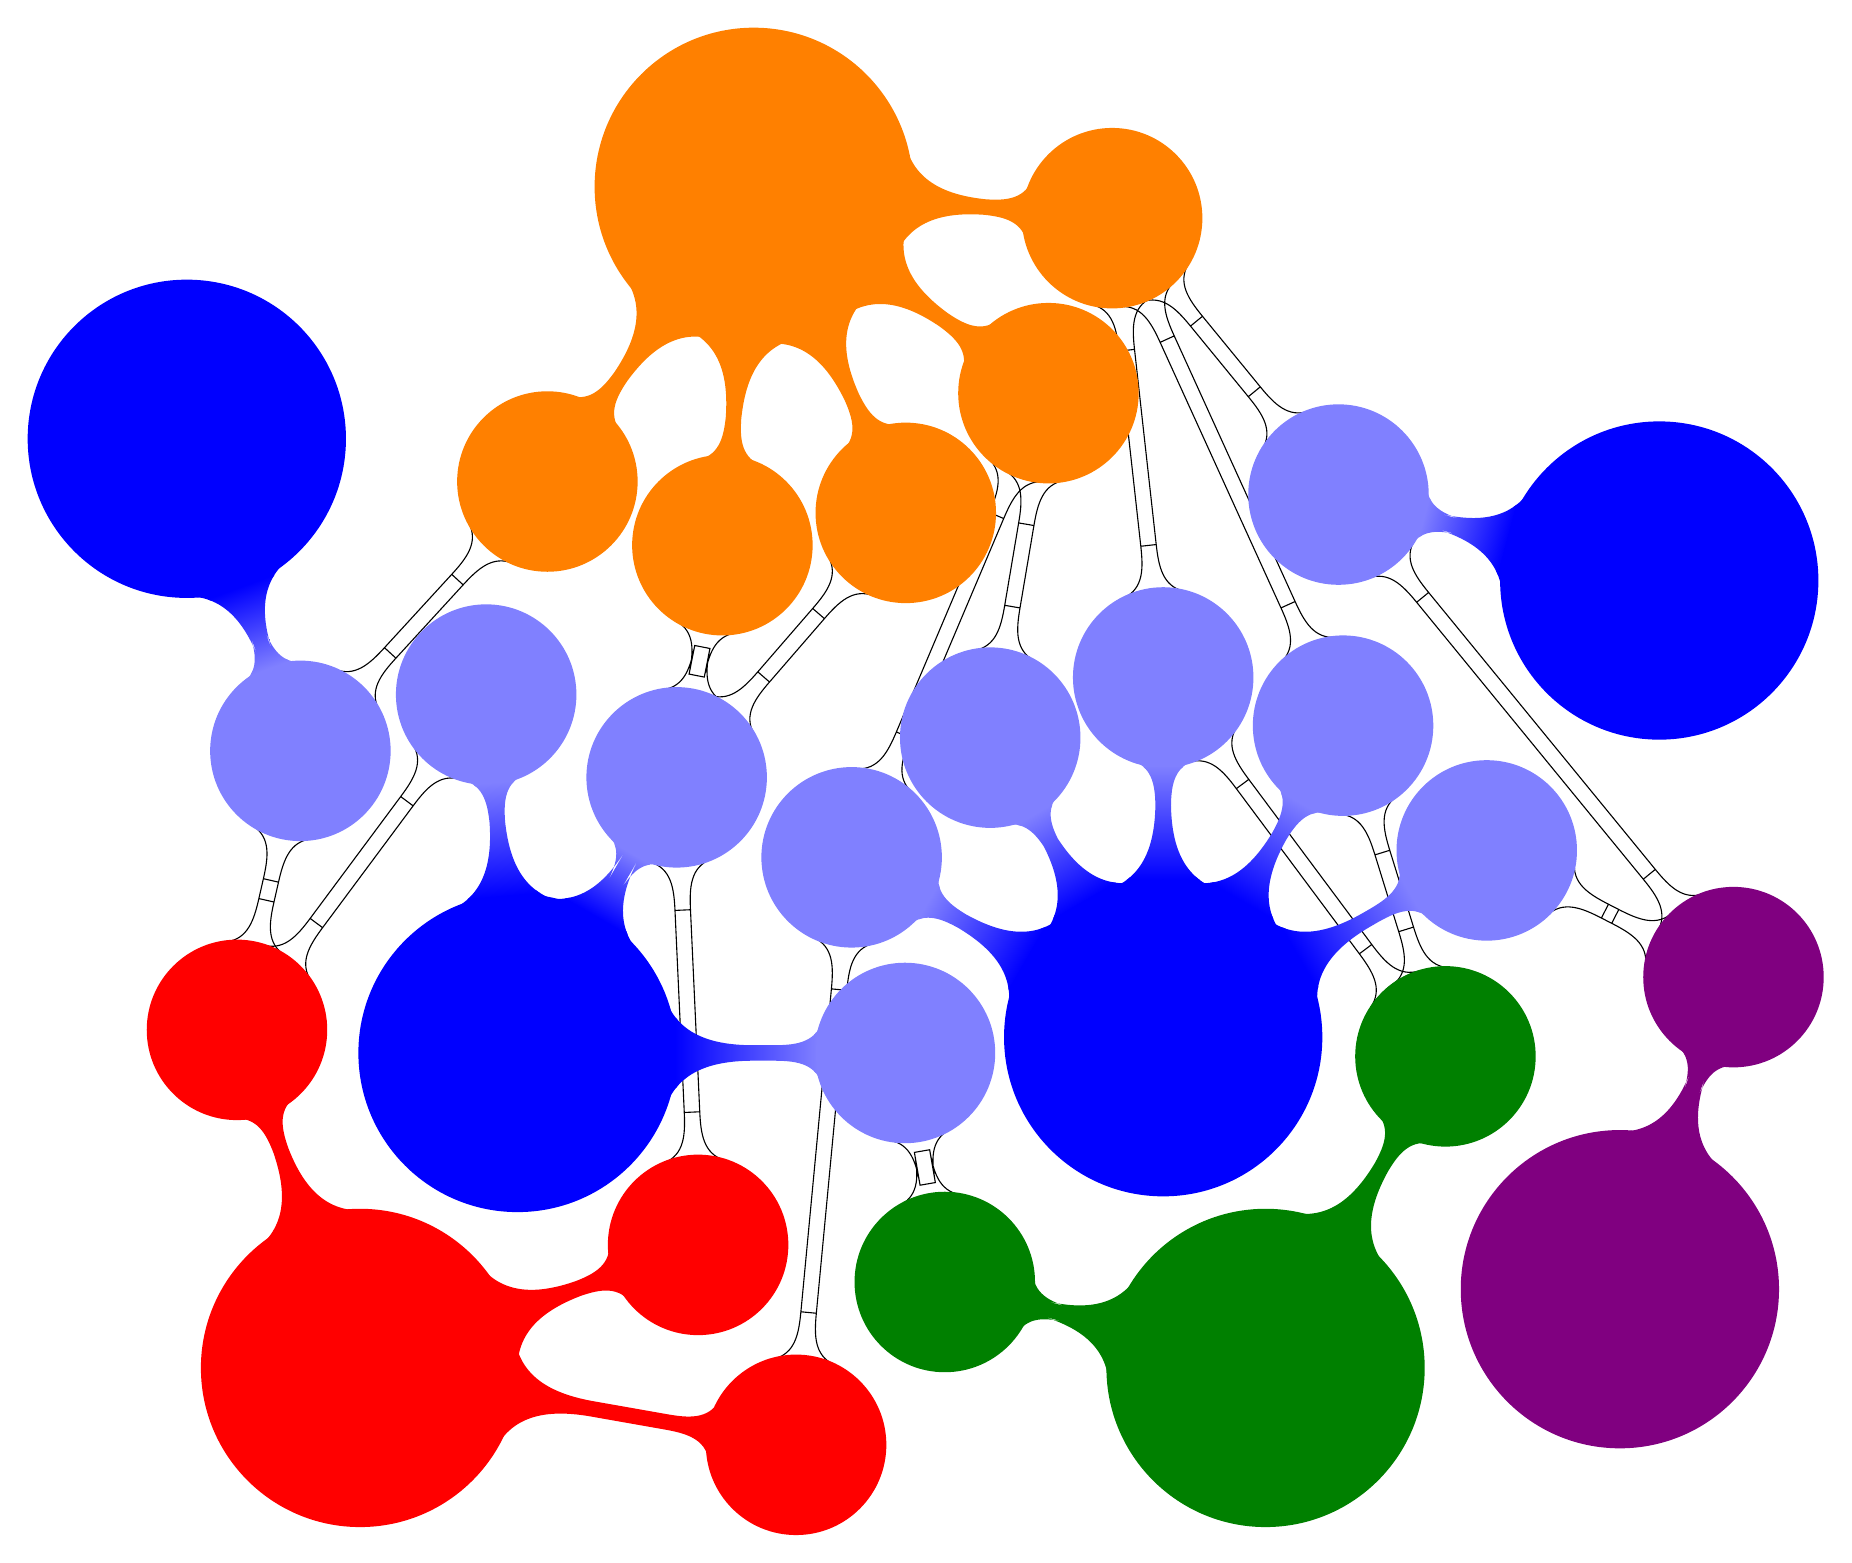
\begin{tikzpicture}[mindmap,
		level 1 concept/.append style={level distance=130,sibling angle=30},
		extra concept/.append style={color=blue!50,text=black}]

	% Applied area: computer science and its subfields

	\begin{scope}[mindmap, concept color=orange, text=white]
		\node [concept] {}[clockwise from=-5]
		child {node [concept] (alg) {}}
		child {node [concept] (cod) {}}
		child {node [concept] (img) {}}
		child {node [concept] (opt) {}}
		child {node [concept] (res) {}};
	\end{scope}

	% Applied area: theoretical physics and its subfields

	\begin{scope}[mindmap, concept color=red,text=white]
		\node [concept] at (-5,-15) {}
		child [grow=-10, level distance=160]
			{node [concept] (qin) {}}
		child [grow=20]
			{node [concept] (csm) {}}
		child [grow=110]
			{node [concept] (mat) {}};
	\end{scope}

	% Applied area: biology and its subfields

	\begin{scope}[mindmap, concept color=green!50!black,text=white]
		\node [concept] at (6.5,-15) {}
		child [grow=165, level distance=120]
			{node [concept] (med) {}}
		child [grow=60]
			{node [concept] (gen) {}};
	\end{scope}

	% Applied area: economics (one subfield)

	\begin{scope}[mindmap, concept color=violet, text=white]
		\node [concept] at (11,-14) {}
		child [grow=70, level distance=120]
			{node [concept] (dec) {}};
	\end{scope}

	% Researchers listed by their main specialization in mathematics

	\begin{scope}[mindmap, concept color=blue]

		% Combinatorics and discrete mathematics 
		\node [concept, text=white] at (5.2,-10.8)
		{}
		[clockwise from=150]
		child [concept color=blue!50] {node [concept] (ver) {}}
		child [concept color=blue!50, level distance=125]
			{node [concept] (kab) {}}
		child [concept color=blue!50]
			{node [concept] (kch) {}}
		child [concept color=blue!50] {node [concept] (raf) {}}
		child [concept color=blue!50, level distance=135]
			{node [concept] (ksh) {}};

		% Partial differential equations
		\node [concept, text=white] at (-3,-11)
		{}
		child [concept color=blue!50, grow=0, level distance=140]
			{node [concept] (lhc) {}}
		child [concept color=blue!50, grow=60, level distance=115]
			{node [concept] (otr) {}}
		child [concept color=blue!50, grow=95] {node [concept] (ndr)
				{}};

		% Probability
		\node [concept, text=white] at (-7.2,-3.2) {}
		child [concept color=blue!50, grow=-70, level distance=120]
			{node [concept] (rbk) {}};

		% Logic
		\node [concept, text=white] at (11.5,-5) {}
		child [concept color=blue!50, grow=165, level distance=120]
			{node [concept] (sht) {}};
	\end{scope}

	% Connections of researchers to applied subfields

	\begin{pgfonlayer}{background}
		\draw [circle connection bar]
		(kab) edge (cod)
		(kch) edge (alg) edge (gen)
		(lhc) edge (med)
		(ksh) edge (dec)
		(ndr) edge (mat)
		(otr) edge (opt) edge (csm) edge (img)
		(raf) edge (alg) edge (gen)
		(rbk) edge (res) edge (mat)
		(sht) edge (alg) edge (dec)
		(ver) edge (qin) edge (cod);
	\end{pgfonlayer}
\end{tikzpicture}

\end{document}
